% arara: pdflatex

\documentclass[tikz,border=0pt]{standalone}
\usepackage{pgfplots}
\usepackage{xcolor}

\begin{document}

\begin{tikzpicture}
% width is 8.64cm
%\newcommand{\figwidth}{8.64cm}
% JFM width and golden ratio
\newcommand{\figwidth}{13.49cm}
\newcommand{\figheight}{6.00cm}
\draw[use as bounding box, white] (0,0) rectangle (\figwidth,\figheight);

% Setup
\begin{scope}[
    xshift=-0.075cm,
    yshift=0.0cm,
    ]
    \node[inner sep=0pt, anchor=south west]  at (0,0)
        {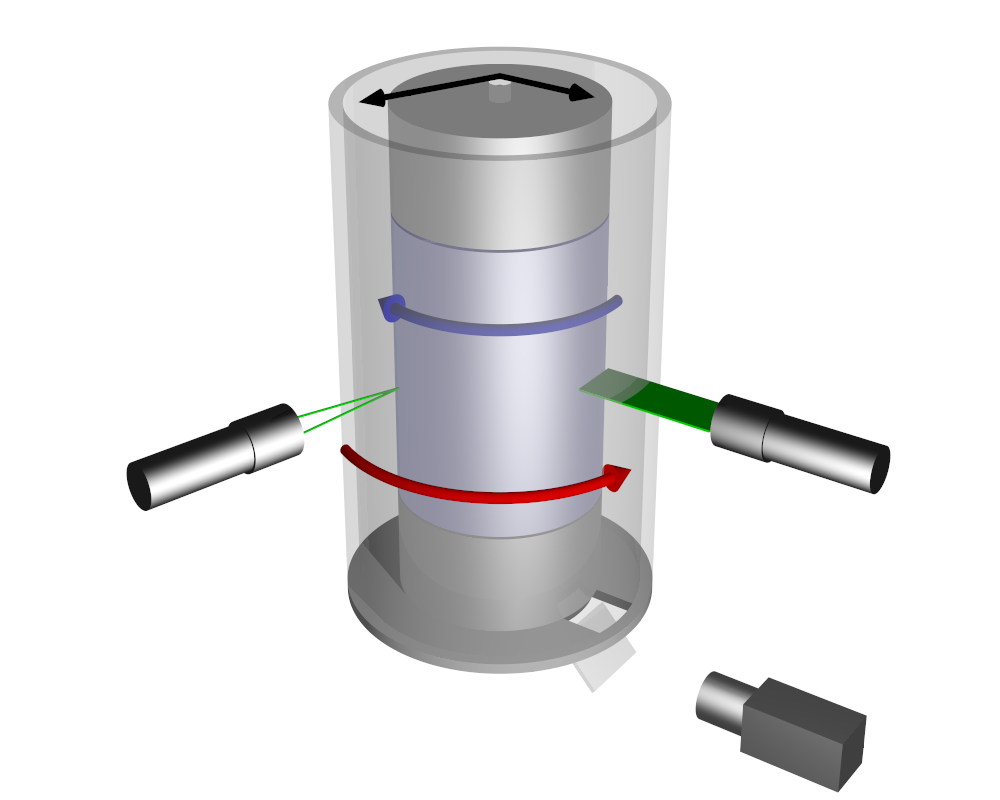
\includegraphics[
            height=6.35cm,
            trim={4.1cm, 0.25cm, 3.8cm, 0}, 
            clip
        ]{t3csetup.png}};
    \node at (3.00, 3.90) {\large$\omega_i$};
    \node at (3.00, 2.60) {\large$\omega_o$};
    \node at (3.50, 5.85) {\large$r_i$};
    \node at (2.40, 5.83) {\large$r_o$};
\end{scope}

\begin{scope}[
    xshift=\figwidth/2 + 0.1cm,
    yshift=1.30cm,
    ]
    \node[inner sep=0pt, anchor=south west]  at (0,0)
        {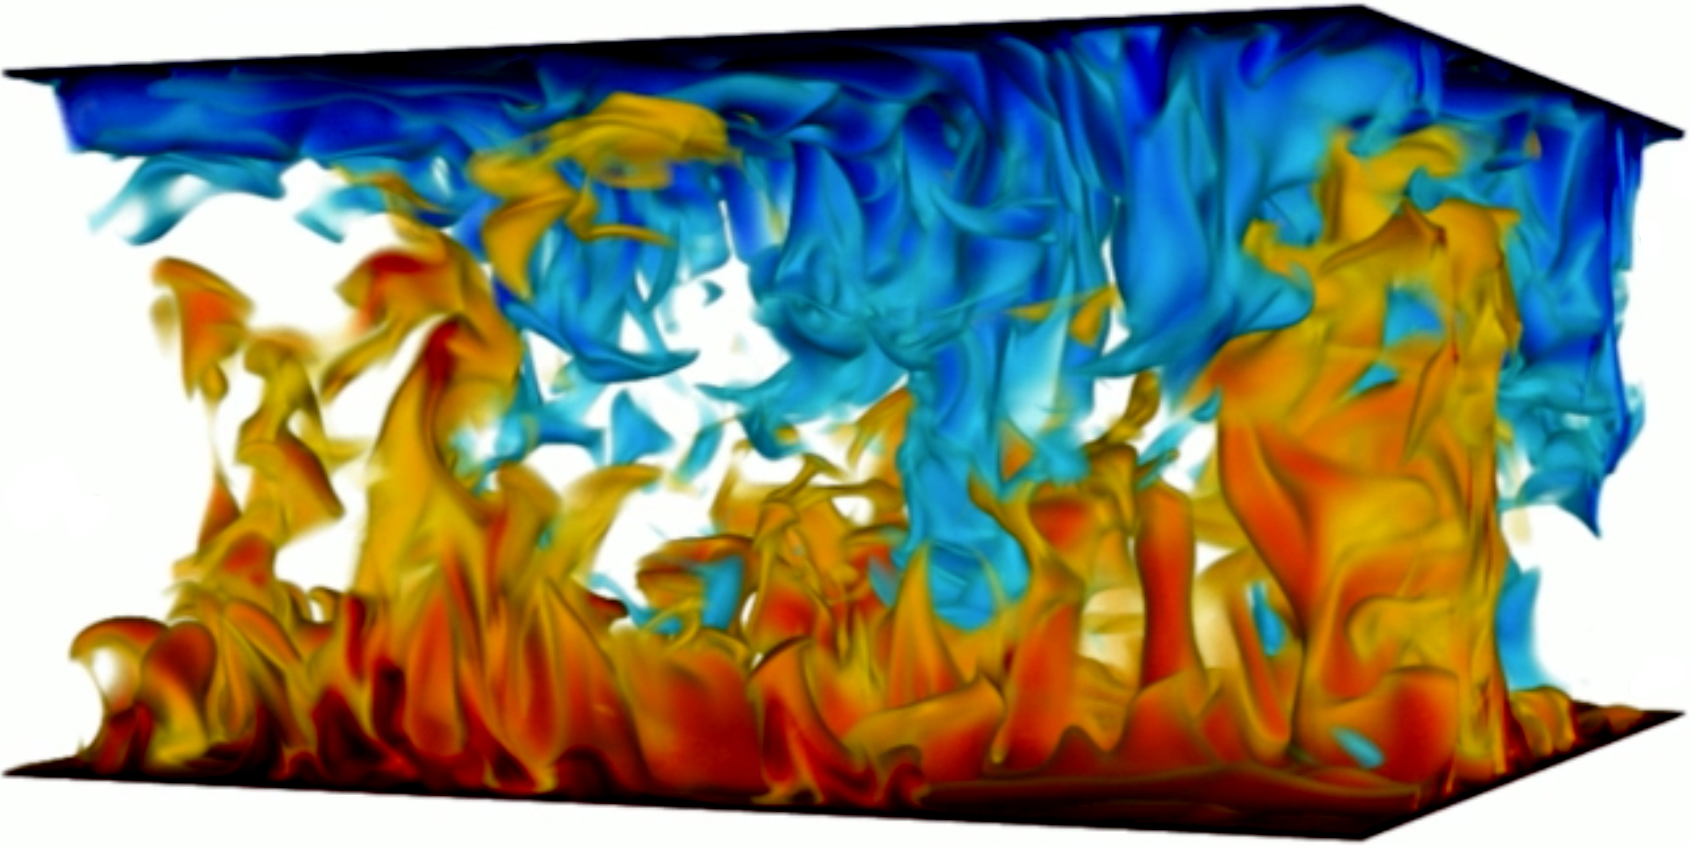
\includegraphics[
            width=6.60cm,
            % trim={4.1cm, 0.25cm, 3.8cm, 0}, 
            clip
        ]{rbc.png}};
        
    \node at (5.25cm, 3.45cm) (5) {};
    \node at (6.70cm, 2.90cm) (6) {};
    \path[
       black,
       <->,
       thick,
       >=latex
       ] (5) edge node [above] {$y$} (6);

    \node at (-0.05cm, 3.14cm) (7) {};
    \node at (5.45cm, 3.40cm) (8) {};
    \path[
       black,
       <->,
       thick,
       >=latex
       ] (7) edge node [above] {$x$} (8);

    \node at (-0.00cm, 3.10cm) (9) {};
    \node at (-0.00cm, 0.20cm) (10) {};
    \path[
       black,
       <->,
       thick,
       >=latex
       ] (9) edge node [left] {$h$} (10);

    % \node at (2.60, 3.50) {\large$\omega_i$};
    % \node at (3.2, 5.18) {\large$r_i$};
    % \node at (2.00, 5.15) {\large$r_o$};
\end{scope}

% % Still image
% \begin{scope}[
%     xshift=8.7cm,
%     yshift=2.80cm
%     ]
%     \node[inner sep=0pt] (image) at (0,0)
%     {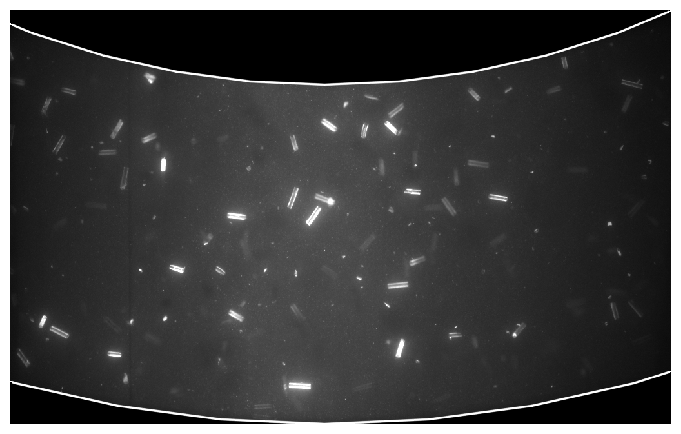
\includegraphics[height=5cm]{figure2image.pdf}};
% \end{scope}

    
% labels
\node at (0.20cm, 5.75cm) {a)};
\node at (6.65cm, 5.75cm) {b)};
% \node at (13.00cm, 5.15cm) {c)};
% \node at (13.90cm, 2.20cm) {d)};


\end{tikzpicture}
\end{document}
